\section{Waves in passive media}\label{sec:waves}

\subsection{A slab of a passive medium}

Consider a plane wave crossing a slab of thickness $L$ of a linear,
homogeneous, isotropic and temporally dispersive medium with relative
permittivity $\epsilon(\omega)$ and permeability $\mu_r(\omega)$. We
consider the propagation factor of a single pass and ignore reflections at
the faces, which is exact for an impedance-matched slab and otherwise
describes the field inside the medium. In our convention the factor is
\[
H(\omega)=\exp\Big(\frac{i\omega n(\omega)L}c\Big),\qquad
n=\sqrt{\epsilon\mu_r}=n_r+in_i .
\]
Passivity of the medium means that $z\epsilon(z)$ and $z\mu_r(z)$ are
Herglotz functions and that $\epsilon$ and $\mu_r$ tend to $1$ as
$z\to i\infty$ \cite{nussenzveig,gustafsson,bernland}. Reality of the fields
makes $\epsilon$ and $\mu_r$ real on $i\R_+$, so that $z\epsilon(z)$ and
$z\mu_r(z)$ lie on the closed positive imaginary axis there.\footnote{Analyticity in $\Cp$ is
causality of the constitutive relations; $\Im(\omega\epsilon(\omega))\ge0$ for
real $\omega$ is the absence of gain; the limit expresses that every medium is
transparent at very high frequency. The Herglotz property in $\Cp$ follows from
these boundary properties by the Poisson representation of the harmonic
function $\Im(z\epsilon(z))$.}

\begin{lemma}\label{lem:index}
$h(z)=zn(z)L/c$ is a Herglotz function with $h(iy)\in i\R$ and
$h(-\bar z)=-\overline{h(z)}$, and its linear coefficient in
\eqref{eq:foster} is $\beta=L/c$. Hence $H=e^{ih}$ is a zero-free passive
system with $\sigma=1$, phase $\varphi=\omega n_rL/c$ and attenuation
$\alpha=\omega n_iL/c$.
\end{lemma}

\begin{proof}
Put $f(z)=z\epsilon(z)$ and $g(z)=z\mu_r(z)$, so that $zn(z)=\sqrt{f(z)g(z)}$.
For $z\in\Cp$, $\arg f$ and $\arg g$ lie in $[0,\pi]$; we take the square
root with argument $\frac12(\arg f+\arg g)\in[0,\pi]$, which is analytic and
is the branch with $n\to1$. So $zn(z)$ maps $\Cp$ to the closed upper
half-plane. On $i\R_+$, $f$ and $g$ lie on $i\R_+$, so their product is
negative and $zn$ lies on $i\R_+$. The symmetry follows from that of $f$ and
$g$, and $\beta=\lim h(iy)/(iy)=L/c$ because $n(iy)\to1$.
\end{proof}

The coefficient $\beta=L/c$ is the vacuum delay: no signal crosses the slab
faster than light. It drops out of the bound, as every delay does.

\begin{theorem}\label{thm:slab}
Let the medium be passive, with $n$ continuous and nonzero on a
neighbourhood of $[a,b]$ in $\overline{\Cp}$, and suppose that on the band
\begin{equation}\label{eq:anomalous}
n_r(\omega)=n_0+\frac C\omega,\qquad a\le\omega\le b,
\end{equation}
with constants $n_0\in\R$ and $C\ge0$. Then
\begin{equation}\label{eq:slab}
\frac1{b-a}\int_a^b\omega\,n_i(\omega)\dd\omega\ \ge\ C\,\Lambda ,
\end{equation}
with equality if and only if the Herglotz measure of $zn(z)$ is carried by
$S$.
\end{theorem}

\begin{proof}
By \cref{lem:index}, $H$ is zero-free, passive and regular on the band, with
phase $\varphi=\omega n_rL/c=CL/c+(n_0L/c)\,\omega$. \Cref{thm:main} with
$\theta=CL/c$ and $\tau=n_0L/c$ gives
$\frac1{b-a}\int\omega n_iL/c\ge(CL/c)\Lambda$, and $L/c$ cancels.
\end{proof}

The thickness of the slab has dropped out: \eqref{eq:slab} is a property of
the material. The condition \eqref{eq:anomalous} says that the phase index
exceeds the group index $n_g=\dd(\omega n_r)/\dd\omega=n_0$ by $C/\omega$, or
equivalently that $\dd n_r/\dd\omega=-C/\omega^2<0$. So
\cref{thm:slab} is a quantitative form of the old observation that
anomalous dispersion requires absorption \cite{kronig,kramers,nussenzveig}:
an index falling like $C/\omega$ across a band requires the frequency-weighted
extinction $\omega n_i$ to be at least $C\Lambda$ on average. In terms of the
intensity absorption coefficient $a_{\rm abs}=2\omega n_i/c$ the bound reads
$\overline{a_{\rm abs}}\ge2C\Lambda/c$.

\begin{figure}[t]
\centering
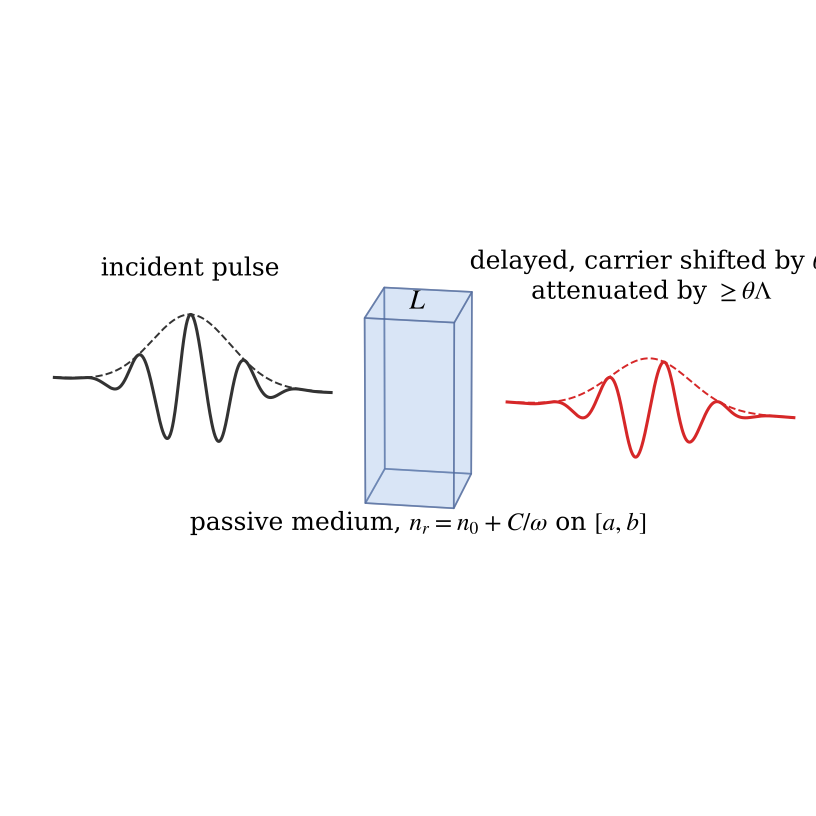
\includegraphics[width=\columnwidth]{figures/fig_slab.png}
\caption{Schematic of \cref{thm:slab}. A pulse crosses a slab of a passive
medium whose index falls like $n_0+C/\omega$ on the band. The envelope is
delayed by $n_0L/c$, the carrier is shifted under it by $\theta=CL/c$, and the
pulse leaves attenuated (the factor is exaggerated). By \cref{thm:slab}
the mean of $\omega n_i$ over the band is at least $C\Lambda$, whatever the
thickness $L$.}
\label{fig:slab}
\end{figure}

\subsection{Approximate constant phase}

The sum rule is linear in the phase, so the bound is stable under
perturbations. Put $P=\int_a^b\abs{p(\omega)}\dd\omega$.

\begin{corollary}\label{cor:stable}
Let $H$ be zero-free, passive and regular on the band, with
$\abs{\varphi(\omega)-\theta-\tau\omega}\le\varepsilon$ on $[a,b]$. Then
\[
\frac1{b-a}\int_a^b\alpha\dd\omega\ \ge\ \theta\Lambda-\frac{P}{2(b-a)}\,\varepsilon .
\]
In particular a zero-free system that is lossless on the band cannot
approximate a constant phase lag $\theta>0$ to within
$\varepsilon<\theta J/P$.
\end{corollary}

\begin{proof}
By \cref{thm:sumrule} and \cref{lem:moments}(i),
$\int_a^b\alpha\ge\frac12\int_a^b\varphi p=\frac12\theta J
+\frac12\int_a^b(\varphi-\theta-\tau\omega)p$, and the last term is at least
$-\frac12\varepsilon P$. If $\alpha=0$ on the band, then
$0\ge\frac12(\theta J-\varepsilon P)$.
\end{proof}

For an octave $J/P=0.2584$, so a lossless zero-free system cannot hold its
phase within $0.258\,\theta$ of any $\theta+\tau\omega$ with $\theta>0$ across
the octave; for the decade $[1,10]$ the ratio is $0.617$. The ratio $J/P$
does not depend on the scale of the band.

\begin{remark}[Broadband phase shifters]\label{rem:darlington}
Broadband ``$90^\circ$ phase shifters'' are pairs of lossless all-pass
networks whose phases differ by approximately $\pi/2$ across a band
\cite{darlington}. Each phase is increasing (\cref{prop:foster}); only their
difference is nearly constant. This is consistent with \cref{cor:stable}:
what the theorem forbids is a lossless network whose own phase is nearly
constant on the band, and a pair of networks never needs one. A device that
shifts a single signal by $\theta$ without a reference channel must lose
transmitted power.
\end{remark}

\subsection{What the bound means for energy}\label{sec:energy}

On the band the power transmission is $T(\omega)=\abs{H(\omega)}^2
=e^{-2\alpha(\omega)}$.

\begin{proposition}\label{prop:energy}
Let $H$ be as in \cref{thm:main} with $\theta>0$.
\begin{enumerate}
\item[(i)] There is $\omega_1\in[a,b]$ with $T(\omega_1)\le e^{-2\theta\Lambda}$,
and for every $\varepsilon>0$ there is a signal with spectrum in
$[-b,-a]\cup[a,b]$ that loses at least the fraction
$1-e^{-2\theta\Lambda}-\varepsilon$ of its energy.
\item[(ii)] The geometric mean of $T$ over the band is at most
$e^{-2\theta\Lambda}$.
\item[(iii)] In a quantised description, a single quantum of frequency
$\omega_1$ fails to be transmitted with probability at least
$1-e^{-2\theta\Lambda}$, and the mean energy it removes from the transmitted
channel is at least $(1-e^{-2\theta\Lambda})\hbar\omega_1$.
\item[(iv)] For a narrow band of relative width $\Delta f/f$ and
$\theta$ in degrees,
$1-e^{-2\theta\Lambda}=\frac{\pi^2}{720}\,\theta\,\frac{\Delta f}f\,
\big(1+O(\theta\Delta f/f)+O((\Delta f/f)^2)\big)$.
\end{enumerate}
\end{proposition}

\begin{proof}
(i) The mean of the continuous function $\alpha$ is at least $\theta\Lambda$,
so $\alpha(\omega_1)\ge\theta\Lambda$ at some $\omega_1$. A signal whose
spectrum is concentrated near $\pm\omega_1$ transmits a fraction of its
energy arbitrarily close to $T(\omega_1)$ by Parseval's identity and the
continuity of $T$. (ii) is \cref{cor:worst}. (iii) A linear lossy element
acts on a single quantum as a beam splitter coupling the transmitted mode
to the other modes of the device; the quantum is transmitted with
probability $T(\omega_1)$. (iv) By \eqref{eq:narrow}, $\Lambda=\frac\pi8\frac{\Delta f}{f}
(1+O((\Delta f/f)^2))$, and $\theta$ degrees are $\pi\theta/180$ radians, so
$2\theta\Lambda=\frac{\pi^2}{720}\theta\frac{\Delta f}f(1+\cdots)$; finally
$1-e^{-x}=x(1+O(x))$.
\end{proof}

The bound is on transmission. The power that is not transmitted may be
absorbed, reflected or routed to other ports, and \cref{prop:energy} does not
say which: a scalar transfer function sees only the output channel. For the
impedance-matched slab of \cref{thm:slab}, which reflects nothing and has no
other port, all of it is absorbed. The energy that is lost is not the
``energy of the phase shift''. A phase
factor is energy neutral (\cref{prop:static}). The loss is the price that
causality and passivity attach to producing that factor on a band.

\subsection{The 5\,MHz example done correctly}

Take the example of \cite{tb23}: a $1^\circ$ phase shift of a wave at
$5$\,MHz, and give it a band, $4.5$ to $5.5$\,MHz, so $\Delta f/f=0.2$. Then
$\kappa=0.1$ and
\begin{gather*}
\Lambda=0.078836,\\
\theta\Lambda=\frac\pi{180}\Lambda=1.3760\times10^{-3}\,\text{Np}
=0.011951\,\text{dB}.
\end{gather*}
A passive device that shifts the carrier--envelope phase by $1^\circ$
across this band therefore fails to transmit at least $0.275\%$ of the power
at its worst frequency, $1-e^{-2\theta\Lambda}=2.748\times10^{-3}$, against
$2.742\times10^{-3}$ from \cref{prop:energy}(iv). A quantum of
$hf=3.313\times10^{-27}$\,J at that frequency removes from the output on average at least
$9.10\times10^{-30}$\,J. This happens to be close to the value
$hf/360=9.20\times10^{-30}$\,J that a phase slipping by $1^\circ$ per period
would remove (\cref{prop:slip}), but the agreement is accidental: the ratio
of the two numbers is $0.989$, close to
$\frac{\pi^2}2\frac{\Delta f}f=0.987$ by \cref{prop:energy}(iv), and it
tends to zero with the bandwidth. For a single sinusoid,
$\Delta f=0$ and a delay of $555.6$\,ps does the job without loss.
